% ============================================================
%  CF UpsolveX -- Complete Project & Analytics Documentation
%  Overleaf-compatible | pdfLaTeX | White Theme | v5.0
% ============================================================

\documentclass[11pt, a4paper]{article}

\usepackage[T1]{fontenc}
\usepackage[utf8]{inputenc}

\usepackage[margin=2.4cm, top=2.8cm, bottom=2.8cm]{geometry}
\usepackage{parskip}
\usepackage[table]{xcolor}

% ---- Palette ------------------------------------------------
\definecolor{bg}{HTML}{FFFFFF}
\definecolor{bgcard}{HTML}{F6F8FA}
\definecolor{bgaccent}{HTML}{EFF3F6}
\definecolor{accent}{HTML}{0969DA}
\definecolor{accentwarm}{HTML}{CF222E}
\definecolor{accentgreen}{HTML}{1A7F37}
\definecolor{accentyellow}{HTML}{9A6700}
\definecolor{accentpurple}{HTML}{6639BA}
\definecolor{accentorange}{HTML}{BC4C00}
\definecolor{textprimary}{HTML}{1F2328}
\definecolor{textsecondary}{HTML}{656D76}
\definecolor{border}{HTML}{D0D7DE}
\definecolor{headerbg}{HTML}{0969DA}

\pagecolor{bg}
\color{textprimary}

% ---- Sections -----------------------------------------------
\usepackage{titlesec}
\usepackage{titling}

\titleformat{\section}
  {\color{accent}\large\bfseries}{\color{accent}\thesection.\ }{0em}{}
  [\color{accent}\vspace{2pt}\rule{\linewidth}{1pt}]

\titleformat{\subsection}
  {\color{accentgreen}\normalsize\bfseries}{\color{textsecondary}\thesubsection\ }{0em}{}
  [\color{border}\rule{\linewidth}{0.5pt}]

\titleformat{\subsubsection}
  {\color{accentpurple}\small\bfseries}{}{0em}{\texttt{>> }}

\titlespacing{\section}{0pt}{22pt}{9pt}
\titlespacing{\subsection}{0pt}{13pt}{5pt}
\titlespacing{\subsubsection}{0pt}{9pt}{3pt}

% ---- Header/Footer ------------------------------------------
\usepackage{fancyhdr}
\pagestyle{fancy}
\fancyhf{}
\fancyhead[L]{\color{textsecondary}\footnotesize\texttt{CF UpsolveX}}
\fancyhead[R]{\color{textsecondary}\footnotesize\texttt{Project, Extension \& Analytics Documentation}}
\fancyfoot[C]{\color{textsecondary}\footnotesize\texttt{--- \thepage\ ---}}
\renewcommand{\headrulewidth}{0.5pt}
\renewcommand{\headrule}{\hbox to\headwidth{\color{border}\leaders\hrule height\headrulewidth\hfill}}
\renewcommand{\footrulewidth}{0pt}

% ---- Tables -------------------------------------------------
\usepackage{tabularx}
\usepackage{booktabs}
\usepackage{array}

% ---- Lists --------------------------------------------------
\usepackage{enumitem}
\setlist[itemize]{leftmargin=1.6em,itemsep=2pt,topsep=4pt,
  label={\color{accent}\small$\triangleright$}}
\setlist[enumerate]{leftmargin=1.8em,itemsep=2pt,topsep=4pt,
  label={\color{accentgreen}\bfseries\arabic*.}}

% ---- TikZ ---------------------------------------------------
\usepackage{tikz}
\usetikzlibrary{positioning}

% ---- tcolorbox ----------------------------------------------
\usepackage{tcolorbox}
\tcbuselibrary{skins,breakable,listings}

\tcbset{basebox/.style={
  colback=bgcard,colframe=border,coltitle=textprimary,
  fonttitle=\small\bfseries,boxrule=0.5pt,arc=4pt,
  left=9pt,right=9pt,top=7pt,bottom=7pt,breakable,enhanced}}

\newtcolorbox{infobox}[1][]{basebox,colframe=accent,
  borderline west={3pt}{0pt}{accent},title={#1}}
\newtcolorbox{warningbox}[1][]{basebox,colframe=accentwarm,
  borderline west={3pt}{0pt}{accentwarm},title={#1}}
\newtcolorbox{successbox}[1][]{basebox,colframe=accentgreen,
  borderline west={3pt}{0pt}{accentgreen},title={#1}}
\newtcolorbox{orangebox}[1][]{basebox,colframe=accentorange,
  borderline west={3pt}{0pt}{accentorange},title={#1}}
\newtcolorbox{purplebox}[1][]{basebox,colframe=accentpurple,
  borderline west={3pt}{0pt}{accentpurple},title={#1}}

\newtcblisting{codebox}[1][]{basebox,colback=bgaccent,colframe=border,
  listing only,
  listing options={basicstyle=\ttfamily\footnotesize\color{accentgreen},
    backgroundcolor=\color{bgaccent},breaklines=true,
    showstringspaces=false,keepspaces=true,columns=flexible},
  title={\color{textsecondary}\texttt{#1}},top=5pt,bottom=5pt}

% ---- Hyperref -----------------------------------------------
\usepackage{hyperref}
\hypersetup{colorlinks=true,linkcolor=accent,urlcolor=accent,
  citecolor=accentgreen,pdftitle={CF UpsolveX Documentation}}

\usepackage{multicol}


% ============================================================
\begin{document}
% ============================================================

% ---- Title --------------------------------------------------
\thispagestyle{empty}
\vspace*{0.8cm}

\begin{tcolorbox}[enhanced,colback=headerbg,colframe=headerbg,
  arc=6pt,boxrule=0pt,left=20pt,right=20pt,top=24pt,bottom=24pt,
  shadow={2pt}{-2pt}{0pt}{black!20}]
  \begin{center}
    {\fontsize{42}{50}\selectfont\bfseries\color{white} CF UpsolveX}\\[0.45em]
    {\large\ttfamily\color{white!75!headerbg}
      Complete Project, Extension \& Analytics Documentation}\\[1em]
    \tcbox[colback=white,colframe=white,arc=4pt,boxrule=0pt,
      left=10pt,right=10pt,top=4pt,bottom=4pt,on line]{%
      {\normalsize\bfseries\color{headerbg}
        Track.\enspace Upsolve.\enspace Improve.}}\\[0.65em]
    {\footnotesize\ttfamily\color{white!65!headerbg} v5.0.0 \quad|\quad 2025}
  \end{center}
\end{tcolorbox}

\vspace{1.2cm}

\begin{infobox}[Project Overview]
  \textbf{CF UpsolveX} is a full-stack web platform and Chrome Extension for
  competitive programmers that enforces systematic improvement through
  \textbf{contest tracking}, \textbf{structured upsolving},
  \textbf{visual analytics}, a \textbf{Chrome Extension sidebar} embedded
  directly into Codeforces, and an \textbf{automated email reminder system}
  that actively nudges users to revisit every missed problem after a contest.

  \vspace{0.4em}
  \textbf{Live Website:} \url{https://cfupsolvex.netlify.app}\\
  \textbf{Backend API:} \url{https://cf-upsolvex.onrender.com}\\
  \textbf{Chrome Extension:} Published on Chrome Web Store
\end{infobox}

\vspace{0.7cm}
\setcounter{tocdepth}{2}
{\hypersetup{linkcolor=accent}\tableofcontents}
\newpage

% ============================================================
\section{Problem Statement}
% ============================================================

Most Codeforces users participate in contests, fail several problems, and
never revisit them. This broken cycle leads to repeated mistakes, random
(non-deliberate) practice, and wasted learning opportunities.

\begin{warningbox}[Three Compounding Harms]
  \begin{itemize}
    \item \textbf{Repeated mistakes}---same algorithmic gaps surface contest after contest
    \item \textbf{No structured improvement}---practice is reactive, not deliberate
    \item \textbf{Wasted potential}---every missed problem is a free lesson left unclaimed
  \end{itemize}
\end{warningbox}

CF UpsolveX fills this gap by enforcing a complete improvement loop:
track $\rightarrow$ identify $\rightarrow$ queue $\rightarrow$ visualise $\rightarrow$ remind.

% ============================================================
\section{Proposed Solution \& Core Pillars}
% ============================================================

\begin{multicols}{2}
  \begin{successbox}[Track]
    Fetch every contest and submission automatically via the Codeforces API.
    Detect rated, unrated, virtual, and missed contests.
  \end{successbox}
  \begin{successbox}[Identify]
    Label each problem: \texttt{solved}, \texttt{upsolved},
    \texttt{wrong}, or \texttt{not\_attempted}.
  \end{successbox}
  \columnbreak
  \begin{successbox}[Queue]
    Auto-generate a \textbf{prioritised} upsolve queue from all pending problems
    using recency, difficulty, and attempt history.
  \end{successbox}
  \begin{successbox}[Remind]
    Email users after each contest with their upsolve queue and a direct dashboard link.
  \end{successbox}
\end{multicols}

\begin{purplebox}[Extension]
  A Chrome Extension injects an \textbf{upsolve sidebar} directly into
  Codeforces, showing stats, queue, and priority scores without leaving
  the site. Available for both registered and unregistered users with a
  smart fallback mode.
\end{purplebox}

% ============================================================
\section{Name \& Tagline}
% ============================================================

\begin{center}
\rowcolors{2}{bgcard}{bg}
\begin{tabularx}{0.82\linewidth}{>{\ttfamily\bfseries\color{accent}}l X}
\toprule
\rowcolor{bgaccent}
\color{textsecondary}Part & \color{textsecondary}Meaning \\
\midrule
CF      & Targets Codeforces users directly \\
Upsolve & The key learning behaviour in competitive programming \\
X       & Symbolises multiplication of growth and performance \\
\bottomrule
\end{tabularx}
\end{center}

\begin{center}
{\Large\bfseries\color{accentwarm} Track.\quad Upsolve.\quad Improve.}
\end{center}

% ============================================================
\section{Tech Stack}
% ============================================================

\begin{center}
\rowcolors{2}{bgcard}{bg}
\begin{tabularx}{0.97\linewidth}{>{\bfseries\color{accent}}l >{\ttfamily\color{accentgreen}}l X}
\toprule
\rowcolor{bgaccent}
\color{textsecondary}Layer    &\color{textsecondary}Technology &\color{textsecondary}Purpose \\
\midrule
Frontend  & React + Vite          & Modular UI with per-component CSS \\
Backend   & FastAPI (Python)      & REST API, scheduler, email dispatch \\
Database  & Supabase (PostgreSQL) & Users, contests, problems, email state \\
Auth      & Supabase Auth         & JWT session management + handle verification \\
Charts    & Recharts              & Analytics visualisations \\
Email     & Brevo (SMTP API)      & Transactional email delivery via HTTP API \\
Templates & Jinja2                & HTML email template rendering \\
Scheduler & APScheduler           & Periodic contest sync \& email triggers (every 30 min) \\
Caching   & cachetools (TTLCache) & In-memory cache for user problem data (10 min TTL) \\
Extension & Chrome MV3            & Content script + service worker sidebar on Codeforces \\
External  & Codeforces API        & Contest, submission, rating, and problem data \\
Hosting   & Netlify + Render      & Frontend on Netlify, backend on Render \\
\bottomrule
\end{tabularx}
\end{center}

% ============================================================
\section{System Architecture}
% ============================================================

\begin{center}
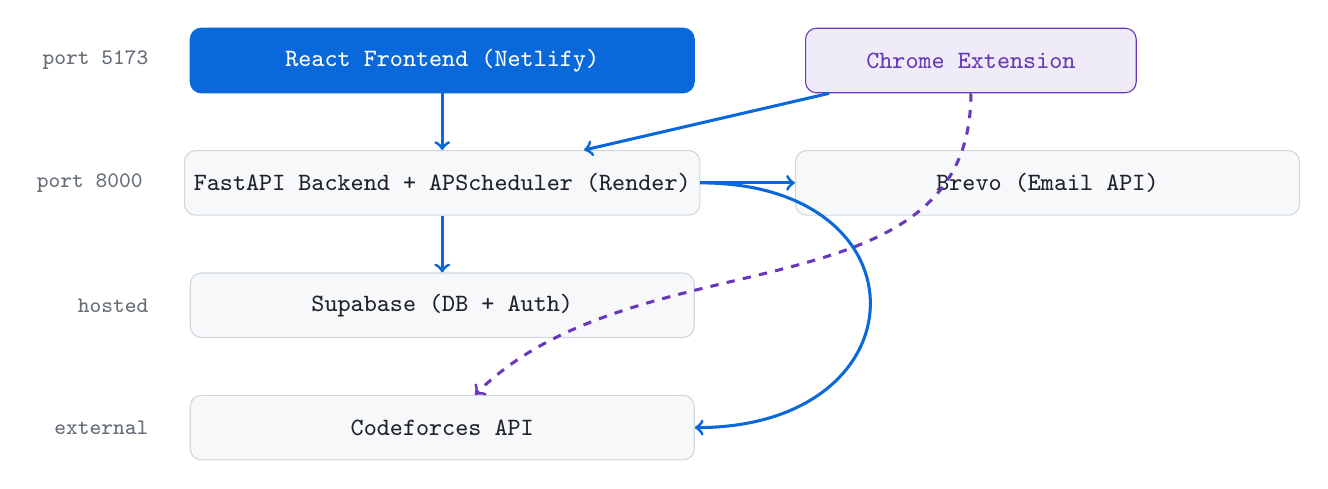
\begin{tikzpicture}[
  node distance=0.72cm,
  box/.style={rectangle,rounded corners=4pt,minimum width=6.4cm,
    minimum height=0.82cm,draw=border,fill=bgcard,
    text=textprimary,font=\small\ttfamily,align=center},
  topbox/.style={rectangle,rounded corners=4pt,minimum width=6.4cm,
    minimum height=0.82cm,draw=accent,fill=accent,
    text=white,font=\small\ttfamily\bfseries,align=center},
  extbox/.style={rectangle,rounded corners=4pt,minimum width=4.2cm,
    minimum height=0.82cm,draw=accentpurple,fill=accentpurple!10,
    text=accentpurple,font=\small\ttfamily\bfseries,align=center},
  arr/.style={->,color=accent,line width=1.1pt},
  lbl/.style={font=\footnotesize\ttfamily,text=textsecondary}
]
  \node[topbox] (fe) {React Frontend (Netlify)};
  \node[extbox,right=1.4cm of fe] (ext) {Chrome Extension};
  \node[box,below=of fe] (be) {FastAPI Backend + APScheduler (Render)};
  \node[box,below=of be] (db) {Supabase (DB + Auth)};
  \node[box,below=of db] (cf) {Codeforces API};
  \node[box,right=1.2cm of be] (em) {Brevo (Email API)};

  \draw[arr] (fe) -- (be);
  \draw[arr] (ext) -- (be);
  \draw[arr] (be) -- (db);
  \draw[arr] (be.east) to[out=0,in=0,looseness=2.4] (cf.east);
  \draw[arr] (be) -- (em);
  \draw[arr,dashed,color=accentpurple] (ext) to[out=-90,in=45] (cf);

  \node[lbl,left=0.4cm of fe] {port 5173};
  \node[lbl,left=0.4cm of be] {port 8000};
  \node[lbl,left=0.4cm of db] {hosted};
  \node[lbl,left=0.4cm of cf] {external};
\end{tikzpicture}
\end{center}

\begin{infobox}[Extension Dual Mode]
  The Chrome Extension connects to the backend API for registered users
  (solid arrow) and falls back to direct Codeforces API calls for
  unregistered users (dashed arrow), computing priority scores locally.
\end{infobox}

% ============================================================
\section{Authentication \& Handle Verification}
% ============================================================

CF UpsolveX uses \textbf{Supabase Auth} for session management with a custom
\textbf{handle ownership verification} step during signup.

\subsection{Signup Flow}

\begin{enumerate}
  \item User provides email, password, and Codeforces handle.
  \item Backend assigns a \textbf{verification problem} (default: \texttt{4A}).
  \item User must submit \textbf{any invalid code} (causing a Compilation Error) to
        that problem on Codeforces within 10 minutes.
  \item Backend checks the user's 5 most recent submissions via Codeforces API ---
        if a Compilation Error on the verification problem is found within the
        last 10 minutes, ownership is confirmed.
  \item Supabase Auth account is created with admin API, and user profile is
        inserted into the \texttt{users} table.
\end{enumerate}

\begin{codebox}[Handle Verification -- Backend Logic]
async def verify_user_handle(handle, verification_problem="4A"):
    submissions = fetch_recent_submissions(handle, count=5)
    for sub in submissions:
        if time_since(sub) > 600 seconds:
            continue
        if sub.problem matches verification_problem:
            if sub.verdict == "COMPILATION_ERROR":
                return True
    return False
\end{codebox}

\subsection{Login \& Protected Routes}

\begin{itemize}
  \item Login returns a Supabase JWT session token.
  \item All dashboard API routes are \textbf{protected} --- the frontend attaches
        the JWT as a \texttt{Bearer} token in the \texttt{Authorization} header.
  \item Backend middleware (\texttt{verify\_token}) validates the JWT via Supabase
        and additionally verifies that the authenticated user owns the requested data.
  \item Extension API routes are \textbf{public} (no auth required) since the
        extension does not have access to the user's JWT.
\end{itemize}

% ============================================================
\section{Workflow}
% ============================================================

\begin{enumerate}
  \item \textbf{User Signup} --- user registers with CF handle, email, password, and
        verifies handle ownership via Compilation Error submission.
  \item \textbf{Initial Sync} --- backend immediately fetches all data from Codeforces
        for the new user and populates the database.
  \item \textbf{Periodic Sync} --- APScheduler runs \texttt{sync\_all\_users} every 30
        minutes, updating all users' contest and problem data.
\begin{codebox}[Codeforces API calls during sync]
GET /api/user.status?handle={cf_handle}     # All submissions
GET /api/user.rating?handle={cf_handle}     # Rating history (rated contests)
GET /api/user.info?handles={cf_handle}      # User info (rating, rank)
GET /api/contest.list                       # All contests metadata
GET /api/problemset.problems                # All problems with ratings
GET /api/contest.standings?contestId={id}   # Fallback for missing problems
\end{codebox}
  \item \textbf{Participation Detection} --- contests classified as rated, unrated,
        virtual, or missed (see Section~\ref{sec:participation}).
  \item \textbf{Data Processing} --- submissions grouped by contest; each problem
        labelled {\color{accentgreen}\texttt{solved}}, {\color{accentwarm}\texttt{wrong}},
        {\color{accentyellow}\texttt{not\_attempted}}, or {\color{accent}\texttt{upsolved}}.
  \item \textbf{Upsolve Detection} --- problem marked \texttt{upsolved} when accepted
        by a \texttt{PRACTICE} submission after the contest.
  \item \textbf{Completion Percentage} --- per-contest metric computed as
        $\frac{\text{solved} + \text{upsolved}}{\text{total problems}} \times 100$.
  \item \textbf{Email Trigger} --- scheduler checks for new contests every 30 minutes;
        if unsolved problems exist and contest not yet notified, an email is dispatched
        via Brevo and \texttt{last\_notified\_contest\_id} updated.
  \item \textbf{Cache Invalidation} --- after any sync or refresh, the in-memory
        TTLCache is invalidated so subsequent API calls return fresh data.
  \item \textbf{Frontend Display} --- dashboard shows KPI cards, contest cards,
        analytics graphs, upsolve queue, and email notification status.
  \item \textbf{Extension Sidebar} --- Chrome Extension displays top 10 queue items,
        stats, and allows manual refresh directly on Codeforces.
\end{enumerate}

% ============================================================
\section{Core Features}
% ============================================================

% ------------------------------------------------------------
\subsection{Contest Tracking \& Classification}
% ------------------------------------------------------------

The system classifies every contest into one of four categories based on
the user's participation data:

\begin{center}
\rowcolors{2}{bgcard}{bg}
\begin{tabularx}{0.95\linewidth}{>{\bfseries\color{accent}}l >{\ttfamily\color{accentgreen}}l X}
\toprule
\rowcolor{bgaccent}
\color{textsecondary}Category & \color{textsecondary}is\_virtual & \color{textsecondary}Description \\
\midrule
Rated Participated    & false & Contest appears in user's rating history \\
Unrated Participated  & true  & User submitted with CONTESTANT or OUT\_OF\_COMPETITION type \\
Virtual Participated  & true  & User submitted with VIRTUAL type (if \texttt{include\_virtual} is ON) \\
Missed Contest        & null  & Contest happened after user's CF registration but user didn't participate \\
\bottomrule
\end{tabularx}
\end{center}

\begin{infobox}[Missed Contest Cutoff]
  Missed contests are only tracked from the user's \textbf{Codeforces
  registration date} (\texttt{registrationTimeSeconds} from the CF API)
  onwards --- not from the beginning of Codeforces history. This prevents
  database bloat and ensures only relevant contests are shown.
\end{infobox}

% ------------------------------------------------------------
\subsection{Contest Participation Detection}
\label{sec:participation}

The Codeforces API does not expose a direct ``participated'' flag.
Participation is inferred using a \textbf{two-signal approach}.

\subsubsection{Signal 1 -- Rating History (Primary)}

\begin{codebox}[Codeforces API call]
GET /api/user.rating?handle={cf_handle}
\end{codebox}

The rating endpoint returns only \textbf{rated participations} --- the most
reliable signal. If a contest appears in the user's rating history, they
definitively participated and \texttt{is\_virtual} is set to \texttt{false}.

\subsubsection{Signal 2 -- Submission Participant Type (Fallback)}

For unrated rounds and educational contests that do not appear in rating
history, participation is inferred from the \texttt{participantType} field
in submissions:

\begin{infobox}[Participation Detection Rule]
  A submission counts as a participation signal based on
  \texttt{author.participantType}:
  \begin{itemize}
    \item \texttt{CONTESTANT} --- live participation (rated or unrated)
    \item \texttt{OUT\_OF\_COMPETITION} --- live but unrated participation
    \item \texttt{VIRTUAL} --- virtual participation (only if \texttt{include\_virtual} is enabled)
    \item \texttt{PRACTICE} --- post-contest practice (marks upsolves, not participation)
  \end{itemize}
\end{infobox}

\subsubsection{Combined Logic}

\begin{codebox}[Pseudo-code -- robust participation detection]
official_contests = set(rating_history.contest_ids)  # Signal 1
participated = set(official_contests)

for submission in all_submissions:
    ptype = submission.author.participantType
    if ptype in [CONTESTANT, OUT_OF_COMPETITION]:
        participated.add(submission.contestId)
    if include_virtual and ptype == VIRTUAL:
        participated.add(submission.contestId)

# Everything else after registration date = missed
missed = all_finished_contests - participated
    where start_time >= user.registrationTimeSeconds
\end{codebox}

\begin{warningbox}[Remaining Edge Case]
  If a user \textbf{opened} a contest but submitted nothing (e.g.\ read
  problems and left), neither signal fires --- this is an unavoidable
  false negative given the available API data. It is acceptable behaviour:
  a zero-submission participation has no upsolve queue to track.
\end{warningbox}

% ------------------------------------------------------------
\subsection{Contest Detail Page}
% ------------------------------------------------------------

Every contest card links to a \textbf{Contest Detail View} that breaks down
all problems in that contest with their statuses and direct links.

\subsubsection{Problem Table}

\begin{center}
\rowcolors{2}{bgcard}{bg}
\begin{tabularx}{0.95\linewidth}{>{\bfseries\color{accent}}l >{\ttfamily\color{accentpurple}}l >{\ttfamily\color{accentgreen}}l X}
\toprule
\rowcolor{bgaccent}
\color{textsecondary}Problem & \color{textsecondary}Status & \color{textsecondary}Upsolved? & \color{textsecondary}Action \\
\midrule
A & solved        & N/A & Open on CF \\
B & wrong         & No  & Upsolve Now \\
C & upsolved      & Yes & Open on CF \\
D & not\_attempted & No  & Upsolve Now \\
\bottomrule
\end{tabularx}
\end{center}

\subsubsection{Page Features}

\begin{itemize}
  \item \textbf{Filter by status} --- show only \texttt{wrong}, \texttt{not\_attempted},
        or \texttt{upsolved}
  \item \textbf{Sort by index} --- default A $\to$ Z; reversible
  \item \textbf{Direct CF link} --- each row has an ``Open on CF'' button using the
        stored \texttt{problem\_url}
  \item \textbf{Upsolve Now button} --- one-click access for pending problems
  \item \textbf{Contest Completion Badge} --- shows completion inline
  \item \textbf{Email Reminder} --- trigger a reminder email for this specific contest
  \item \textbf{Missed Contest indicator} --- clearly labels contests the user did not participate in
\end{itemize}

% ------------------------------------------------------------
\subsection{Upsolve Tracking \& Priority Queue}
% ------------------------------------------------------------

Problems solved after contest close (via \texttt{PRACTICE} submissions) are
marked \texttt{upsolved}. All remaining unsolved problems populate a
\textbf{prioritised upsolve queue} that serves as the user's daily practice board.

\subsubsection{Queue Prioritization Logic}

With potentially hundreds of pending problems, ordering matters.
CF UpsolveX computes a \textbf{Priority Score} for each pending problem:

\begin{infobox}[Priority Score Formula]
\[
  \text{Priority} = w_1 \cdot \text{RecencyScore} + w_2 \cdot \text{DifficultyScore} + w_3 \cdot \text{AttemptScore}
\]
Where each component uses a mathematically grounded function:
\begin{itemize}
  \item \textbf{RecencyScore} $= e^{-d/30}$ where $d$ = days since contest.
        Exponential decay: 3-day-old contest $\approx 0.90$, 60-day-old $\approx 0.14$
  \item \textbf{DifficultyScore} $= e^{-\Delta^2 / (2\sigma^2)}$ where
        $\Delta = |\text{problem\_rating} - \text{user\_rating}|$ and $\sigma = 300$.
        Gaussian bell curve centred on user's rating; problems near the user's
        level score highest
  \item \textbf{AttemptScore} $= \min(1.0,\; 0.25 \times \text{failed\_attempts})$.
        Linear growth capped at 1.0; more failed attempts = known weak spot
\end{itemize}
\end{infobox}

\begin{codebox}[Default weights]
w1 = 0.50  # Recency  (most important: stay in context)
w2 = 0.30  # Difficulty (prioritise skill-gap problems)
w3 = 0.20  # Failed attempts (target known weak spots)
\end{codebox}

\subsubsection{Score Normalisation}

Raw scores are normalised so the highest-priority problem always shows
\textbf{10.0}:
\[
  \text{NormalisedScore}_i = \frac{\text{RawScore}_i}{\max(\text{RawScores})} \times 10
\]

The queue is sorted descending by normalised score and displayed with
colour-coded priority badges:
{\color{accentwarm}\textbf{HIGH}} ($>7$),
{\color{accentpurple}\textbf{MED}} ($4$--$7$),
{\color{accent}\textbf{LOW}} ($<4$).

% ------------------------------------------------------------
\subsection{Dashboard KPI Cards}
% ------------------------------------------------------------

The dashboard header displays six live metric cards, giving an instant
health-check of the user's progress.

\begin{center}
\rowcolors{2}{bgcard}{bg}
\begin{tabularx}{0.92\linewidth}{>{\bfseries\color{accent}}l X}
\toprule
\rowcolor{bgaccent}
\color{textsecondary}KPI Card & \color{textsecondary}Description \\
\midrule
Pending Upsolves     & Total problems still in the upsolve queue \\
Completed Upsolves   & Total problems successfully upsolved to date \\
Current Streak       & Consecutive days with at least one solve/upsolve \\
Total Contests       & Number of unique contests tracked \\
Solved in Contest    & Cumulative problems solved during live contests \\
Completion Rate \%   & $\frac{\text{solved} + \text{upsolved}}{\text{total problems}} \times 100$ \\
\bottomrule
\end{tabularx}
\end{center}

\subsubsection{Streak Calculation}

The streak system is fully implemented. It counts consecutive calendar days
with at least one problem solved or upsolved:

\begin{codebox}[Streak Logic]
solved_dates = set of dates where user solved/upsolved a problem

if today in solved_dates:
    streak = 1, check backwards from yesterday
elif yesterday in solved_dates:
    streak = 1, check backwards from day-before-yesterday

while current_date in solved_dates:
    streak += 1
    current_date -= 1 day
\end{codebox}

% ------------------------------------------------------------
\subsection{Contest Completion Percentage}
% ------------------------------------------------------------

\begin{orangebox}[The Most Addictive Metric]
  Instead of ``I solved 2 problems'', users see:\\[0.5em]
  \hspace*{2em}\textbf{CF Round 1045 --- Contest Completion: 66\%}\\[0.5em]
  This reframes the goal: finishing a contest becomes a measurable,
  completable task rather than an open-ended struggle.
\end{orangebox}

\subsubsection{Calculation}

\[
  \text{Contest Completion \%} =
  \frac{\text{Solved During Contest} + \text{Upsolved After Contest}}
       {\text{Total Problems in Contest}} \times 100
\]

A contest reaches \textbf{100\%} only when every problem is either solved
or upsolved --- creating a powerful sense of closure.

% ------------------------------------------------------------
\subsection{Graphs \& Progress Analytics}
% ------------------------------------------------------------

Interactive Recharts-powered visualisations with division and index filtering:

\begin{center}
\rowcolors{2}{bgcard}{bg}
\begin{tabularx}{0.92\linewidth}{>{\bfseries\color{accent}}l >{\ttfamily\color{accentpurple}}l X}
\toprule
\rowcolor{bgaccent}
\color{textsecondary}Graph & \color{textsecondary}Type & \color{textsecondary}Insight \\
\midrule
Upsolve Progress         & Line Chart & Daily upsolve count over time \\
Contest Performance      & Bar Chart  & Per-contest solved/upsolved/total breakdown \\
Completion Ratio         & Pie Chart  & Overall solved vs.\ upsolved vs.\ pending split \\
Contest Completion Trend & Line Chart & Completion \% per contest over time \\
\bottomrule
\end{tabularx}
\end{center}

\subsubsection{Analytics Filters}

\begin{itemize}
  \item \textbf{Max Problem Index} --- filter analytics by problem index (A through G, or All)
  \item \textbf{Division Filter} --- filter by contest division: Div.~1, Div.~2, Div.~3,
        Div.~4, Div.~1+2, Educational, or All
  \item Filters apply across all charts simultaneously
\end{itemize}

% ------------------------------------------------------------
\subsection{Email Reminder System}
% ------------------------------------------------------------

\begin{orangebox}[Goal]
  Convert CF UpsolveX from a passive tracker into an \textbf{active learning
  assistant} that reaches out to users after every contest --- so missed
  problems are never silently forgotten.
\end{orangebox}

\subsubsection{Email Provider}

Emails are sent via the \textbf{Brevo} (formerly Sendinblue) transactional
email API using HTTP requests with an API key. Both \textbf{HTML} (rendered
from Jinja2 templates) and \textbf{plain-text} fallback bodies are included.

\subsubsection{Trigger Mechanism}

\begin{itemize}
  \item \textbf{Scheduled (automatic)} --- APScheduler runs
        \texttt{check\_and\_send\_emails} every 30 minutes, checking all users
        with \texttt{email\_enabled = true} for new contests.
  \item \textbf{Manual trigger} --- user can trigger a reminder for a specific
        contest from the Contest Detail page.
\end{itemize}

\subsubsection{Processing Logic}

\begin{codebox}[Pseudo-code -- email scheduler]
for user in users where email_enabled = true:
    new_problems = problems where contest_id > last_notified_contest_id
    participated_contests = problems where is_virtual is not null

    for contest in new_contests:
        if contest in participated_contests:
            compute solved, total, missed, completion%
            build upsolve_queue sorted by problem index
            send_email(user.email, contest_data, upsolve_queue)

    update last_notified_contest_id = max(new_contest_ids)
\end{codebox}

\subsubsection{Email Content}

\begin{codebox}[Subject line]
CF UpsolveX -- Don't Skip Your Missed Problems
\end{codebox}

The email body includes a beautifully rendered HTML template (via Jinja2)
showing contest name, solve stats, completion percentage, and up to 5
priority-ordered problems with ratings and attempt counts. A direct
dashboard link is included for one-click access.

\subsubsection{Anti-Spam Protection}

\begin{itemize}
  \item \textbf{One email per contest} --- \texttt{last\_notified\_contest\_id} prevents duplicates
  \item \textbf{First-sync protection} --- on initial registration, \texttt{last\_notified\_contest\_id}
        is set to the user's maximum contest ID, preventing a flood of emails for historical contests
  \item \textbf{User opt-out} --- \texttt{email\_enabled} toggle in Settings
\end{itemize}

% ------------------------------------------------------------
\subsection{User Settings Page}
% ------------------------------------------------------------

A dedicated \texttt{/settings} page allows users to manage their account
preferences and notification behaviour.

\begin{center}
\rowcolors{2}{bgcard}{bg}
\begin{tabularx}{0.92\linewidth}{>{\bfseries\color{accent}}l X >{\ttfamily\color{accentgreen}}l}
\toprule
\rowcolor{bgaccent}
\color{textsecondary}Setting & \color{textsecondary}Description & \color{textsecondary}Default \\
\midrule
Change CF Handle          & Update Codeforces username; triggers full re-sync & --- \\
Change Email              & Update notification email address & --- \\
Email Notifications       & Toggle all email reminders on / off & ON \\
Weekly Digest             & Receive a weekly summary email & ON \\
Include Virtual Contests  & Count virtual participations in stats and queue & OFF \\
Max Problem Index         & Only track problems up to this index (A--G or All) & Z \\
\bottomrule
\end{tabularx}
\end{center}

\begin{infobox}[Smart Re-sync on Settings Change]
  Changing CF handle, max problem index, or include virtual triggers an
  automatic \textbf{background re-sync} via \texttt{BackgroundTasks} ---
  the user doesn't need to manually refresh.
\end{infobox}

% ------------------------------------------------------------
\subsection{Caching Layer}
% ------------------------------------------------------------

To reduce database load and improve response times, the backend implements
an \textbf{in-memory TTL cache} using the \texttt{cachetools} library.

\begin{itemize}
  \item \textbf{Cache scope:} per-user problem status list (including joined contest data)
  \item \textbf{Max entries:} 100 users
  \item \textbf{TTL:} 600 seconds (10 minutes)
  \item \textbf{Invalidation:} explicit invalidation on refresh/sync via
        \texttt{invalidate\_user\_cache(user\_id)}
  \item \textbf{Pagination:} the \texttt{fetch\_all} helper bypasses Supabase's
        1000-row limit by paginating automatically
\end{itemize}

% ============================================================
\section{Chrome Extension}
% ============================================================

The CF UpsolveX Chrome Extension brings the upsolve queue directly into
the Codeforces website via a slide-in sidebar --- no tab switching needed.

\subsection{Architecture}

\begin{center}
\rowcolors{2}{bgcard}{bg}
\begin{tabularx}{0.95\linewidth}{>{\bfseries\color{accent}}l >{\ttfamily\color{accentgreen}}l X}
\toprule
\rowcolor{bgaccent}
\color{textsecondary}Component & \color{textsecondary}File & \color{textsecondary}Role \\
\midrule
Manifest        & manifest.json  & Chrome MV3 config; permissions, content scripts \\
Service Worker  & background.js  & API calls, data fetching, alarm-based periodic sync \\
Content Script  & content.js     & Sidebar injection, UI rendering, user interaction \\
Styles          & content.css    & Dark-themed sidebar styling with CSS variables \\
Popup           & popup.html     & Extension popup with logo and dashboard link \\
\bottomrule
\end{tabularx}
\end{center}

\subsection{Permissions}

\begin{codebox}[manifest.json -- key fields]
"manifest_version": 3,
"permissions": ["storage", "alarms"],
"host_permissions": [
  "*://*.codeforces.com/*",
  "https://cf-upsolvex.onrender.com/*"
],
"content_scripts": [{
  "matches": ["*://*.codeforces.com/*"],
  "css": ["content.css"],
  "js": ["content.js"],
  "run_at": "document_end"
}]
\end{codebox}

\subsection{Navbar Button}

The extension injects a styled \textbf{``CF UpsolveX''} button into the
Codeforces top navigation bar. The button features:

\begin{itemize}
  \item Blue text with a glowing border that matches the CF aesthetic
  \item A subtle \textbf{breathing glow animation} that pulses every 2.5 seconds
  \item Brighter glow on hover for visual feedback
  \item Clicking toggles the sidebar open/closed
\end{itemize}

\subsection{Sidebar UI}

The sidebar slides in from the right edge of the screen with a smooth
cubic-bezier animation. It features a dark theme with glassmorphism
effects and contains:

\subsubsection{Header}

\begin{itemize}
  \item \textbf{Title} with gradient text (``CF UpsolveX'')
  \item \textbf{Subtitle} --- ``TRACK $\bullet$ UPSOLVE $\bullet$ IMPROVE''
  \item \textbf{Refresh button} --- triggers a full sync with Codeforces via
        the public \texttt{POST /api/extension/refresh/\{handle\}} endpoint
  \item \textbf{Max Index dropdown} --- filter queue by problem index (A through G, or All)
  \item \textbf{Close button} with 90\textdegree{} rotation animation on hover
\end{itemize}

\subsubsection{Stats Widget}

A 2$\times$2 grid showing four key metrics:
\textbf{Pending} upsolves,
\textbf{Completion} rate \%,
\textbf{Upsolved} count, and
\textbf{Streak} in days.

\subsubsection{Queue List}

Top 10 priority-ordered problems, each showing:
\begin{itemize}
  \item Problem ID and name (e.g.\ ``2234D -- Problem'')
  \item Rating and division badge (Div.~1, Div.~2, Div.~3, Div.~4, Edu, Global)
  \item Colour-coded priority badge with score
  \item Clickable --- opens problem in a \textbf{new tab}
\end{itemize}

\subsubsection{Footer}

Shows ``Showing X of Y Pending Problems'' count and a ``View Full Queue''
button linking to the main CF UpsolveX dashboard.

\subsection{Handle Detection}

The extension automatically detects the logged-in Codeforces user by
parsing the DOM:

\begin{codebox}[Handle detection]
const userLinks = document.querySelectorAll(
  '.lang-chooser a[href^="/profile/"]'
);
cfHandle = userLinks[0].href.split('/profile/')[1];
\end{codebox}

If no handle is found (user logged out), the sidebar shows an
``Authentication Required'' state with a registration link.

\subsection{Dual-Mode Data Fetching}

\begin{center}
\rowcolors{2}{bgcard}{bg}
\begin{tabularx}{0.95\linewidth}{>{\bfseries\color{accent}}l X}
\toprule
\rowcolor{bgaccent}
\color{textsecondary}Mode & \color{textsecondary}Behaviour \\
\midrule
Registered User   & Fetches from \texttt{GET /api/extension/queue/\{handle\}}.
                    Returns server-computed priority queue, full stats, and KPIs. \\
Unregistered User & Falls back to direct Codeforces API calls
                    (\texttt{user.info} + \texttt{user.status}). Computes
                    priority scores locally in the service worker.
                    Stats show ``N/A'' for unavailable metrics. \\
\bottomrule
\end{tabularx}
\end{center}

\subsection{Background Sync}

The service worker sets up a Chrome alarm (\texttt{syncData}) that runs
every 6 hours to refresh cached data in \texttt{chrome.storage.local}.
Data is also refreshed on every page load.

% ============================================================
\section{Database Schema}
% ============================================================

\subsubsection{Users Table}

\begin{center}
\rowcolors{2}{bgcard}{bg}
\begin{tabularx}{0.97\linewidth}{>{\ttfamily\color{accentgreen}}l >{\ttfamily\color{accent}}l X}
\toprule
\rowcolor{bgaccent}
\color{textsecondary}Column &\color{textsecondary}Type &\color{textsecondary}Notes \\
\midrule
id                          & UUID      & Primary key (from Supabase Auth) \\
cf\_handle                  & TEXT      & Unique Codeforces username \\
email                       & TEXT      & For email reminders \\
rating                      & INT       & Current CF rating (synced from API) \\
rank                        & TEXT      & Current CF rank (e.g.\ ``pupil'', ``expert'') \\
cf\_info                    & JSONB     & Full Codeforces user.info response (avatar, etc.) \\
last\_notified\_contest\_id & INT       & Prevents duplicate email notifications \\
email\_enabled              & BOOLEAN   & Master toggle for all email reminders \\
weekly\_digest              & BOOLEAN   & Weekly summary email preference \\
min\_notify\_index          & TEXT      & Maximum problem index to track (default: Z = all) \\
include\_virtual            & BOOLEAN   & Include virtual contest participations in stats \\
created\_at                 & TIMESTAMP & Account creation time \\
\bottomrule
\end{tabularx}
\end{center}

\subsubsection{Contests Table}

\begin{center}
\rowcolors{2}{bgcard}{bg}
\begin{tabularx}{0.95\linewidth}{>{\ttfamily\color{accentgreen}}l >{\ttfamily\color{accent}}l X}
\toprule
\rowcolor{bgaccent}
\color{textsecondary}Column &\color{textsecondary}Type &\color{textsecondary}Notes \\
\midrule
contest\_id          & INT       & Codeforces contest identifier (upsert key) \\
name                 & TEXT      & Contest display name \\
start\_time          & TIMESTAMP & Contest start time (UTC) \\
end\_time            & TIMESTAMP & Contest end time (UTC) \\
total\_problems      & INT       & Total number of problems in the contest \\
\bottomrule
\end{tabularx}
\end{center}

\subsubsection{User Problem Status Table \textnormal{\small(Core Table)}}

\begin{center}
\rowcolors{2}{bgcard}{bg}
\begin{tabularx}{0.97\linewidth}{>{\ttfamily\color{accentgreen}}l >{\ttfamily\color{accent}}l X}
\toprule
\rowcolor{bgaccent}
\color{textsecondary}Column &\color{textsecondary}Type &\color{textsecondary}Notes \\
\midrule
id              & UUID      & Primary key \\
user\_id        & UUID      & Foreign key $\to$ users.id \\
contest\_id     & INT       & Foreign key $\to$ contests.contest\_id \\
problem\_index  & TEXT      & Problem label (A, B, C, D1, etc.) \\
problem\_rating & INT       & Codeforces difficulty rating \\
problem\_url    & TEXT      & Direct CF problem URL \\
status          & ENUM      & solved / wrong / not\_attempted / upsolved \\
failed\_attempts& INT       & Count of wrong submissions \\
solved\_at      & TIMESTAMP & Nullable; set when solved or upsolved \\
is\_virtual     & BOOLEAN   & \texttt{false} = rated, \texttt{true} = unrated/virtual, \texttt{null} = missed \\
\bottomrule
\end{tabularx}
\end{center}

\begin{infobox}[Composite Upsert Key]
  The table uses a composite unique constraint on
  \texttt{(user\_id, contest\_id, problem\_index)} for upsert operations,
  ensuring no duplicate problem entries per user per contest.
\end{infobox}

% ============================================================
\section{API Design}
% ============================================================

\subsection{Public Routes (No Auth)}

\begin{center}
\rowcolors{2}{bgcard}{bg}
\begin{tabularx}{0.97\linewidth}{>{\ttfamily\bfseries\color{accentwarm}}l >{\ttfamily\color{accent}}l X}
\toprule
\rowcolor{bgaccent}
\color{textsecondary}Method &\color{textsecondary}Endpoint &\color{textsecondary}Description \\
\midrule
POST & /api/auth/signup                    & Register with handle verification \\
POST & /api/auth/login                     & Login; returns JWT session \\
GET  & /api/extension/queue/\{handle\}     & Top 10 queue + stats for extension \\
POST & /api/extension/refresh/\{handle\}   & Trigger CF sync from extension \\
\bottomrule
\end{tabularx}
\end{center}

\subsection{Protected Routes (JWT Required)}

\begin{center}
\rowcolors{2}{bgcard}{bg}
\begin{tabularx}{0.97\linewidth}{>{\ttfamily\bfseries\color{accentwarm}}l >{\ttfamily\color{accent}}l X}
\toprule
\rowcolor{bgaccent}
\color{textsecondary}Method &\color{textsecondary}Endpoint &\color{textsecondary}Description \\
\midrule
GET  & /api/user/\{handle\}              & Fetch user record \\
POST & /api/user/                         & Create user (admin) \\
POST & /api/user/\{handle\}/refresh      & Re-fetch from CF API and update DB \\
GET  & /api/contests/\{handle\}          & Full contest history with per-problem status \\
GET  & /api/contests/\{handle\}/\{id\}   & Detail view for a single contest \\
GET  & /api/upsolve/\{handle\}           & Priority-ordered upsolve queue \\
GET  & /api/analytics/\{handle\}         & All graph data (supports ?max\_index \& ?division filters) \\
GET  & /api/dashboard/\{handle\}         & KPI card metrics \\
POST & /api/notify/\{handle\}            & Manually trigger email reminder \\
GET  & /api/settings/\{handle\}          & Retrieve user settings \\
PUT  & /api/settings/\{handle\}          & Update user settings (triggers re-sync if needed) \\
\bottomrule
\end{tabularx}
\end{center}

% ============================================================
\section{Folder Structure}
% ============================================================

\subsection{Frontend}

\begin{codebox}[frontend/src/ -- React + Vite]
src/
  pages/
    Landing.jsx / Landing.css           # Public landing page
    Auth.jsx / Auth.css                 # Login + Signup with handle verification
    Dashboard.jsx / Dashboard.css       # KPI cards + upcoming contests
    UpsolveQueue.jsx / UpsolveQueue.css # Priority queue with "Upsolve Now"
    Contests.jsx / Contests.css         # Rated/Unrated/Missed contest tabs
    ContestDetail.jsx / ContestDetail.css # Per-contest problem table
    Analytics.jsx / Analytics.css       # Charts with division/index filters
    Settings.jsx / Settings.css         # Account + notification preferences

  components/
    layout/
      Layout.jsx / Layout.css           # Protected route wrapper
      Navbar.jsx                        # Top navigation with profile modal
    charts/
      AnalyticsCharts.jsx / .css        # Recharts-based chart components
    problem/
      PriorityQueue.jsx / .css          # Queue item component
    profile/
      ProfileModal.jsx / .css           # User profile dropdown
    common/
      LoadingScreen.jsx / .css          # Full-screen loading animation
      MultiSelectDropdown.jsx           # Division filter dropdown

  context/
    AuthContext.jsx                     # Supabase auth state management

  services/
    api.js                             # JWT-attached fetch wrapper + cache
    supabase.js                        # Supabase client init
    codeforces.js                      # Direct CF API calls (for landing)

  data/
    cp_tips.js                         # Competitive programming tips

  styles/
    global.css                         # Global styles
    variables.css                      # CSS custom properties
    animations.css                     # Shared animations

  utils/
    alerts.jsx                         # Toast notification helpers

  App.jsx                             # Route definitions
  App.css                             # App-level styles
  main.jsx                            # Entry point with AuthProvider
  index.css                           # Base CSS reset
\end{codebox}

\subsection{Backend}

\begin{codebox}[backend/ -- FastAPI]
backend/
  app/
    main.py                            # FastAPI app, CORS, route registration,
                                       # APScheduler setup (30-min intervals)
    routes/
      auth.py                          # POST /signup, /login (public)
      extension.py                     # GET /queue, POST /refresh (public)
      user.py                          # GET/POST user, POST refresh (protected)
      contest.py                       # GET contest list + detail (protected)
      upsolve.py                       # GET priority queue (protected)
      analytics.py                     # GET chart data with filters (protected)
      dashboard.py                     # GET KPI metrics (protected)
      notify.py                        # POST email trigger (protected)
      settings.py                      # GET/PUT user settings (protected)

    services/
      codeforces.py                    # CF API wrapper (rating, status,
                                       # info, contests, problems, verify)
      processor.py                     # Core sync engine: participation
                                       # detection, problem status mapping,
                                       # contest/problem upsert
      priority_queue.py                # Priority score formula (exp decay,
                                       # Gaussian difficulty, linear attempts)
      completion_service.py            # KPI calculation, index filtering,
                                       # virtual filtering, streak logic
      analytics_service.py             # Chart data generation (pie, bar,
                                       # line, trend)
      contest_detail.py                # Contest history grouping/formatting
      cache_service.py                 # TTLCache (100 users, 10 min TTL)
      email_service.py                 # Brevo API integration + Jinja2
      auth_middleware.py               # JWT verification via Supabase

    scheduler/
      contest_checker.py               # sync_all_users (every 30 min)
      email_trigger.py                 # check_and_send_emails (every 30 min)

    templates/
      reminder_email.html              # Jinja2 HTML email template

    models/
      schemas.py                       # Pydantic models (UserSignup,
                                       # UserLogin, UserBase, etc.)
    db/
      supabase_client.py               # Supabase client + fetch_all helper

  .env                                 # SUPABASE_URL, SUPABASE_KEY,
                                       # BREVO_API_KEY, EMAIL_ADDRESS
  requirements.txt                     # Python dependencies
\end{codebox}

\subsection{Chrome Extension}

\begin{codebox}[extension/ -- Chrome MV3]
extension/
  manifest.json                        # MV3 config, permissions, content scripts
  background.js                        # Service worker: API calls, alarms,
                                       # message handling, fallback mode
  content.js                           # Sidebar injection, navbar button,
                                       # UI rendering, event handlers
  content.css                          # Dark sidebar theme with CSS vars
  popup.html                           # Extension popup (logo + dashboard link)
  icon.png                             # Extension icon (16/48/128)
\end{codebox}

% ============================================================
\section{Future Scope}
% ============================================================

\begin{itemize}
  \item \textbf{AI recommendations} --- suggest next problem by rating gap and topic weakness
  \item \textbf{AI-generated email insights} --- plain-English performance summaries
  \item \textbf{Prediction graphs} --- rating forecast via regression on upsolve and completion trends
  \item \textbf{Multi-platform support} --- CodeChef, LeetCode, AtCoder
  \item \textbf{Weekly digest emails} --- chart snapshots + improvement tips (backend ready)
  \item \textbf{Adaptive priority weights} --- ML-tuned weights per user based on upsolve history
  \item \textbf{Contest comparison} --- side-by-side completion \% for two users (social feature)
  \item \textbf{Daily activity heatmap} --- GitHub-style streak visualisation
  \item \textbf{Topic-wise breakdown} --- identify weak algorithm categories from problem tags
  \item \textbf{Extension enhancements} --- inline problem status badges on CF problem pages
\end{itemize}

% ============================================================
\section{Conclusion}
% ============================================================

\begin{infobox}[Final Summary]
  CF UpsolveX is a \textbf{learning enforcement and visualisation system}
  that ensures contest mistakes are never ignored, progress is always visible,
  and improvement is structurally guaranteed.

  \vspace{0.5em}
  The platform operates across three surfaces:
  \begin{enumerate}
    \item \textbf{Web Dashboard} --- full-featured React application with contest
          tracking, priority queue, analytics charts, and user settings
    \item \textbf{Chrome Extension} --- lightweight sidebar injected directly
          into Codeforces for at-a-glance queue access without leaving the site
    \item \textbf{Email System} --- automated Brevo-powered reminders after every
          contest, converting passive tracking into active accountability
  \end{enumerate}

  \vspace{0.5em}
  The \textbf{handle verification} system ensures account authenticity,
  the \textbf{caching layer} keeps the API fast, and the
  \textbf{Contest Completion Percentage} reframes every contest as a
  completable task, making 100\% the only acceptable finish line.
  Random practice becomes a structured, data-driven, habit-forming engine.
\end{infobox}

\vspace{1em}
\begin{center}
  {\large\bfseries\color{accent} CF UpsolveX}\\[0.3em]
  {\color{textsecondary}``Doesn't just track your mistakes ---}\\
  {\color{textprimary}\bfseries it reminds you to fix them.''}
\end{center}

\vfill
\begin{center}
  \color{border}\rule{0.45\linewidth}{0.5pt}\\[5pt]
  {\footnotesize\ttfamily\color{textsecondary}
    CF UpsolveX \textbullet{} Project, Extension \& Analytics
    \textbullet{} \LaTeX{} v5.0}
\end{center}

\end{document}
